\documentclass[tikz,border=10pt]{standalone}

\begin{document}
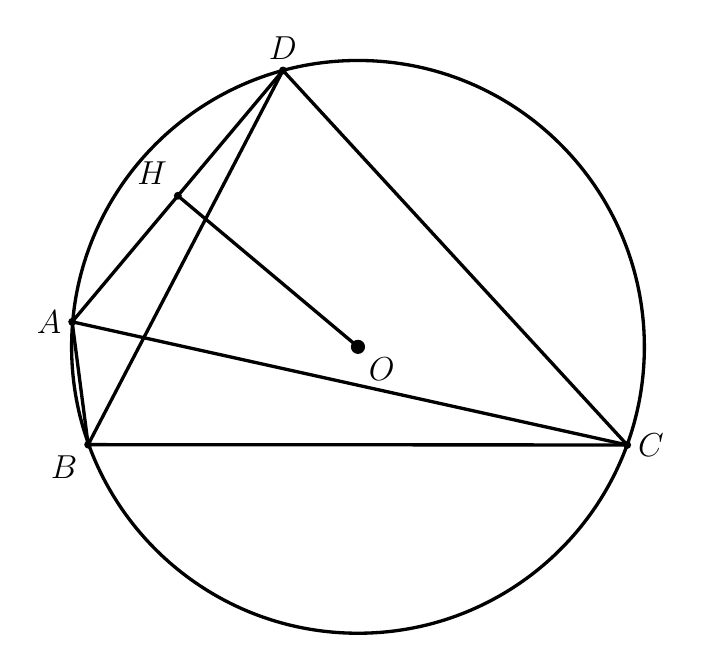
\begin{tikzpicture}[line width=1.2pt, line join=round]
\coordinate (A) at (-3.536,0.104);
\coordinate (B) at (-3.333,-1.456);
\coordinate (C) at (3.513,-1.460);
\coordinate (D) at (-0.859,3.296);
\coordinate (H) at (-2.194,1.705);
\coordinate (O) at (0.094,-0.214);









  
  \draw[line width=1.2pt] (O) circle[radius=3.637];

  
  \draw (A) -- (B);
  \draw (A) -- (C);
  \draw (A) -- (D);
  \draw (B) -- (C);
  \draw (B) -- (D);
  \draw (C) -- (D);

  
  \draw (H) -- (O);

  
  \foreach \p in {A,B,C,D,H}
    \fill (\p) circle (0.050);
  
  \fill (O) circle (0.090);

  
  \node[left,  font=\fontsize{12.5}{15}\selectfont] at (A) {$A$};
  \node[below left,  font=\fontsize{12.5}{15}\selectfont] at (B) {$B$};
  \node[right, font=\fontsize{12.5}{15}\selectfont] at (C) {$C$};
  \node[above, font=\fontsize{12.5}{15}\selectfont] at (D) {$D$};
  \node[above left, font=\fontsize{12.5}{15}\selectfont] at (H) {$H$};
  \node[below right, font=\fontsize{12.5}{15}\selectfont] at (O) {$O$};
\end{tikzpicture}
\end{document}